%%%%%%%%%%%%%%%%%%%%%%%%%%%%%%
\chapter{Besoins fonctionnels et non fonctionnels}
%%%%%%%%%%%%%%%%%%%%%%%%%%%%%%

\section{Besoins fonctionnels}

\subsection{Interface Homme Machine (IHM)}
L'interface Web que nous allons réaliser devra permettre de charger la description d'un réseau pré-existant ou d'en créer un nouveau, mais également de modifier les descriptions de ce dernier.\\
Elle donnera également le moyen à l'utilisateur de saisir les fonctions et options qui l'intéressent puis de lancer les calculs des modes élémentaires de flux du réseau d'intérêt. De plus, un script récurent de commandes pourra être enregistré et chargé par la suite.

\subsection{Chargement des données}
Une zone de chargement de fichiers (de différents formats) à partir du disque dur de l'utilisateur sera présente sur l'interface. \\
Selon le type du fichier donné en paramètre d'entrée, une liste de choix possibles pourra être proposée. Ainsi les résultats d'expériences similaires (suppression, modification des réactifs, produits ou enzymes du réseau) devront pouvoir être comparés avec un affichage en vis-à-vis, ce qui implique une sauvegarde temporaire des résultats sur le serveur. 

\subsection{Réglage des paramètres}
Il sera possible pour un utilisateur confirmé ou habitué à l'interface d'avoir accès à un mode de réglage avancé des paramètres, s'il le désire. Ces derniers seront fixés à des valeurs par défaut pour les débutants. 

\subsection{Résultats}
Enfin, la visualisation des résultats devra apparaître de façon claire et conviviale à l'utilisateur au travers de l'interface Web. De plus, les résultats pourront être exportés dans un fichier pour une analyse ultérieure. Par ailleurs, nous allons essayer de mettre en place un dispositif d'annotations des fichiers.

\subsection{Aide en ligne}
Un message d'aide apparaîtra au survol du curseur de la souris sur la fonction ou l'option choisie. Ainsi l'utilisateur pourra avoir plus d'informations sur la commande concernée.

\subsection{Maquette de l'interface}
Nous avons réalisé une série de maquettes pour avoir une idée du genre d'interface Web que nous voudrions. Elles ont été réalisée avec le logiciel Pencil~\cite{pencil:url} et permettent de mieux illustrer le rendu final de notre projet.

\subsubsection{Page d'accueil}

\begin{figure}[!ht]
	\begin{center}
		\fbox{
   		 \begin{minipage}[c]{0.9\textwidth}
  			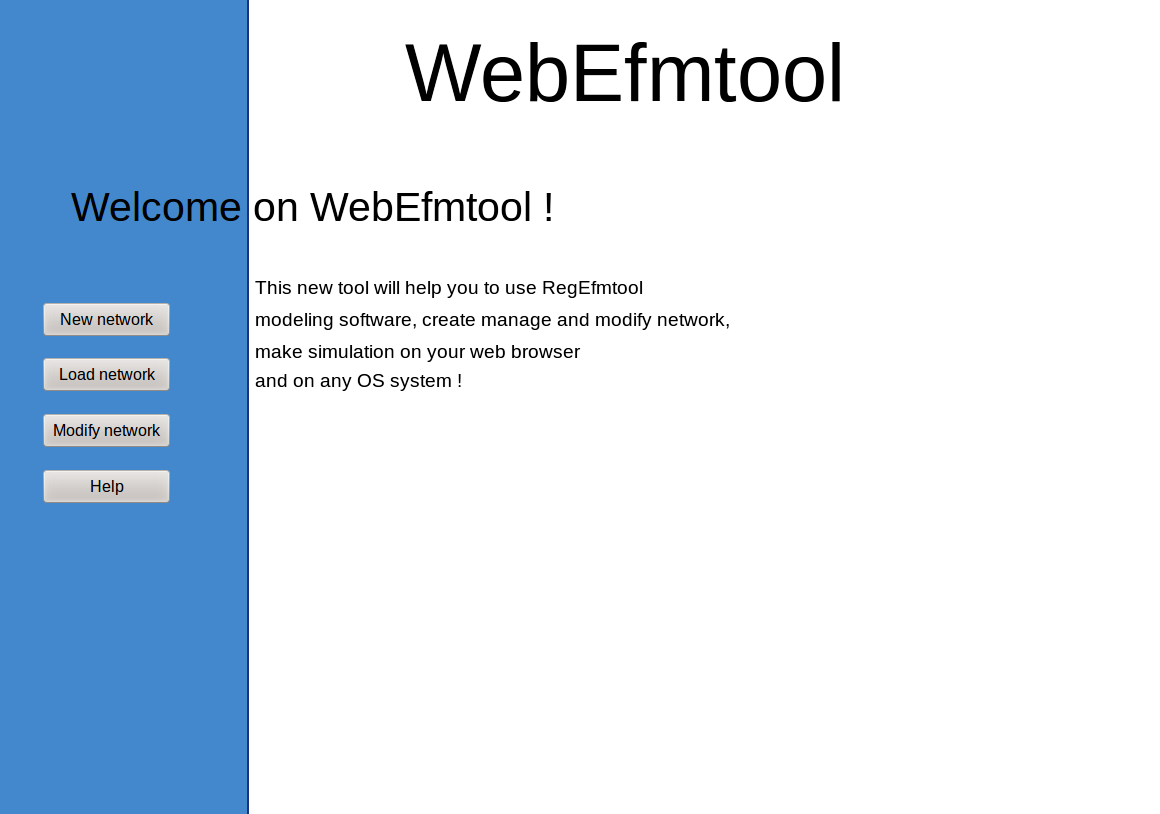
\includegraphics[width=0.90\textwidth]{Accueil.png}  
		 \end{minipage}}
		\caption{Page d'accueil}
  		\label{main}
  	\end{center}	
\end{figure}

Le logiciel \textit{regEfmtool} étant en anglais, nous avons choisi d'utiliser cette même langue pour notre interface. De plus, cela permettra son utilisation par un plus grand nombre d'utilisateurs. \\
			Lors de l'affichage de la page d'accueil (Figure \ref{main}), l'utilisateur aura le choix entre créer un réseau métabolique manuellement, ou bien le charger à partir de fichiers préexistant. 
	
\pagebreak	
			
\subsubsection{Création d'un nouveau réseau}

\begin{figure}[!ht]
	\begin{center}
		\fbox{
   		 \begin{minipage}[c]{0.9\textwidth}
  			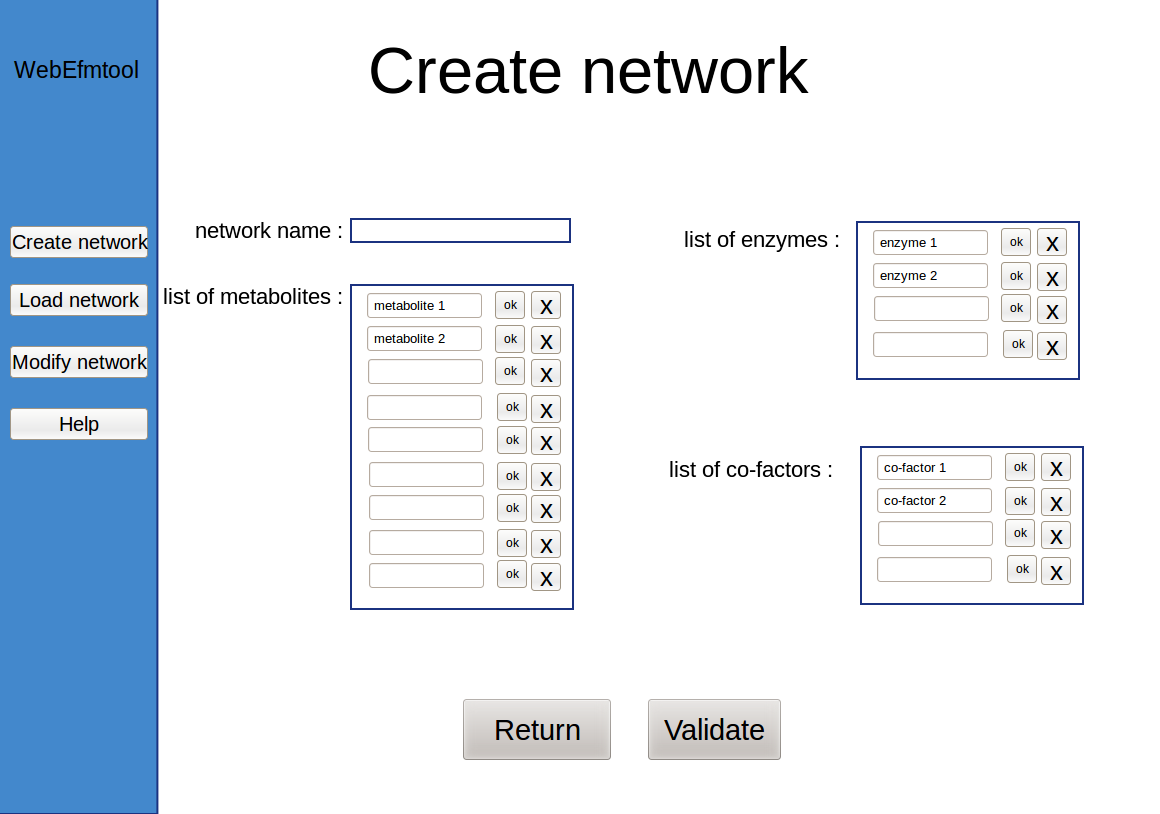
\includegraphics[width=0.90\textwidth]{CreateNetwork.png}  
		 \end{minipage}}
		\caption{Entrée des composants du réseau}
  		\label{reseau}
  	\end{center}	
\end{figure}

Si l'utilisateur clique sur le bouton de création d'un nouveau réseau métabolique (Figure \ref{reseau}), une première page Web s'affichera. Il devra rentrer les noms de tous les métabolites et enzymes participant aux réactions, ainsi que celui du réseau. Il aura la possibilité de valider ou supprimer chaque métabolite et enzyme. Dans le cas d'une validation, les données seront récupérées afin de générer automatiquement les fichiers nécessaires au fonctionnement du logiciel.

\pagebreak

\begin{figure}[!ht]
	\begin{center}
		\fbox{
   		 \begin{minipage}[c]{0.9\textwidth}
  			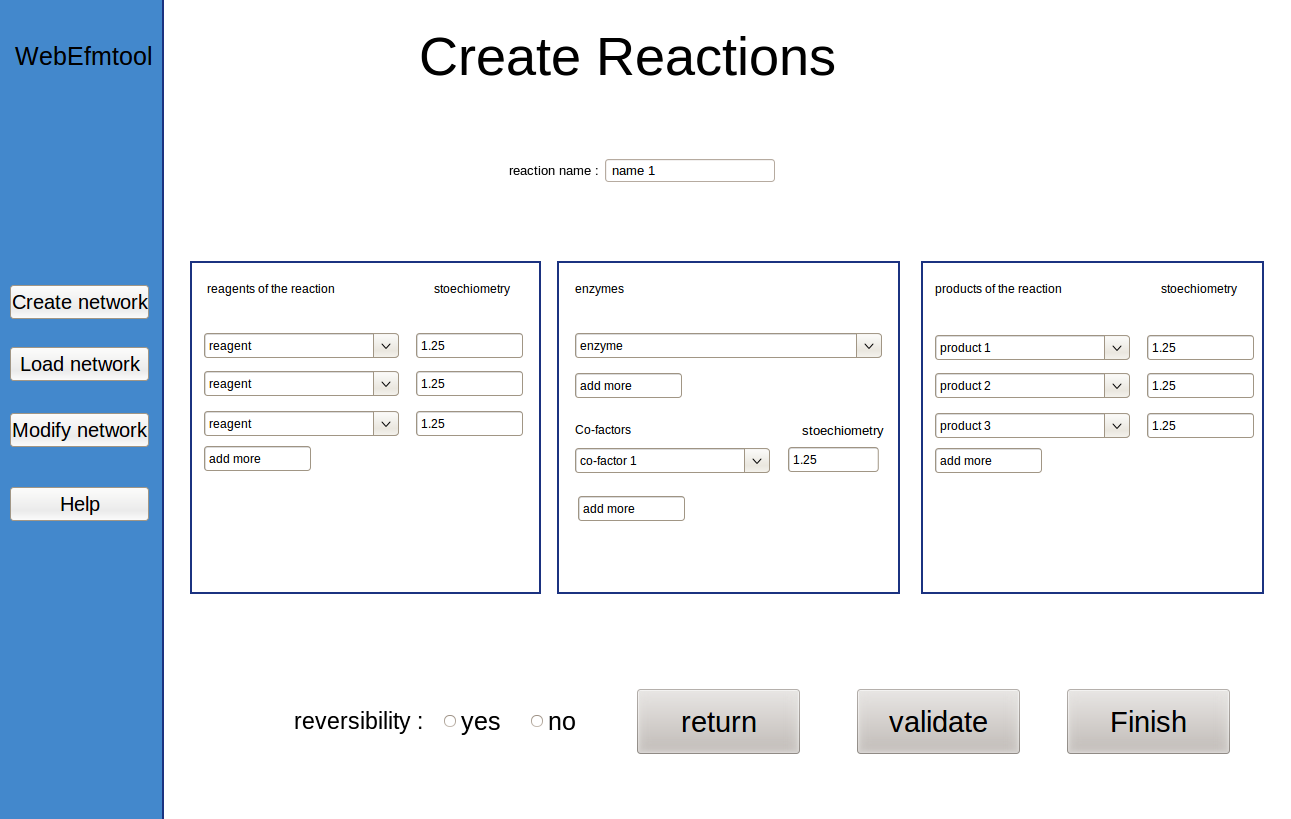
\includegraphics[width=0.90\textwidth]{CreateReac.png}  
		 \end{minipage}}
		\caption{Création des réactions}
  		\label{reactions}
  	\end{center}	
\end{figure}

Une fois les noms des composants du réseau métabolique entrés, l'utilisateur va devoir créer les réactions une à une (Figure \ref{reactions}). Tout d'abord, il devra s'occuper des réactifs de la réaction: un menu déroulant lui donnera le choix entre tous les métabolites qu'il a saisi précédemment et il n'aura plus qu'à entrer le coefficient stœchiométrique associé. Il en sera de même pour les enzymes (sans le coefficient de stœchiométrie dans ce cas), les produits et les co-facteurs. Pour ce qui est de la réversibilité des réactions, il suffira de cocher la bonne case. L'utilisateur pourra ensuite ajouter une réaction ou valider son réseau. 

\pagebreak

\subsubsection{Chargement d'un réseau préexistant}

\begin{figure}[!ht]
	\begin{center}
		\fbox{
   		 \begin{minipage}[c]{0.9\textwidth}
  			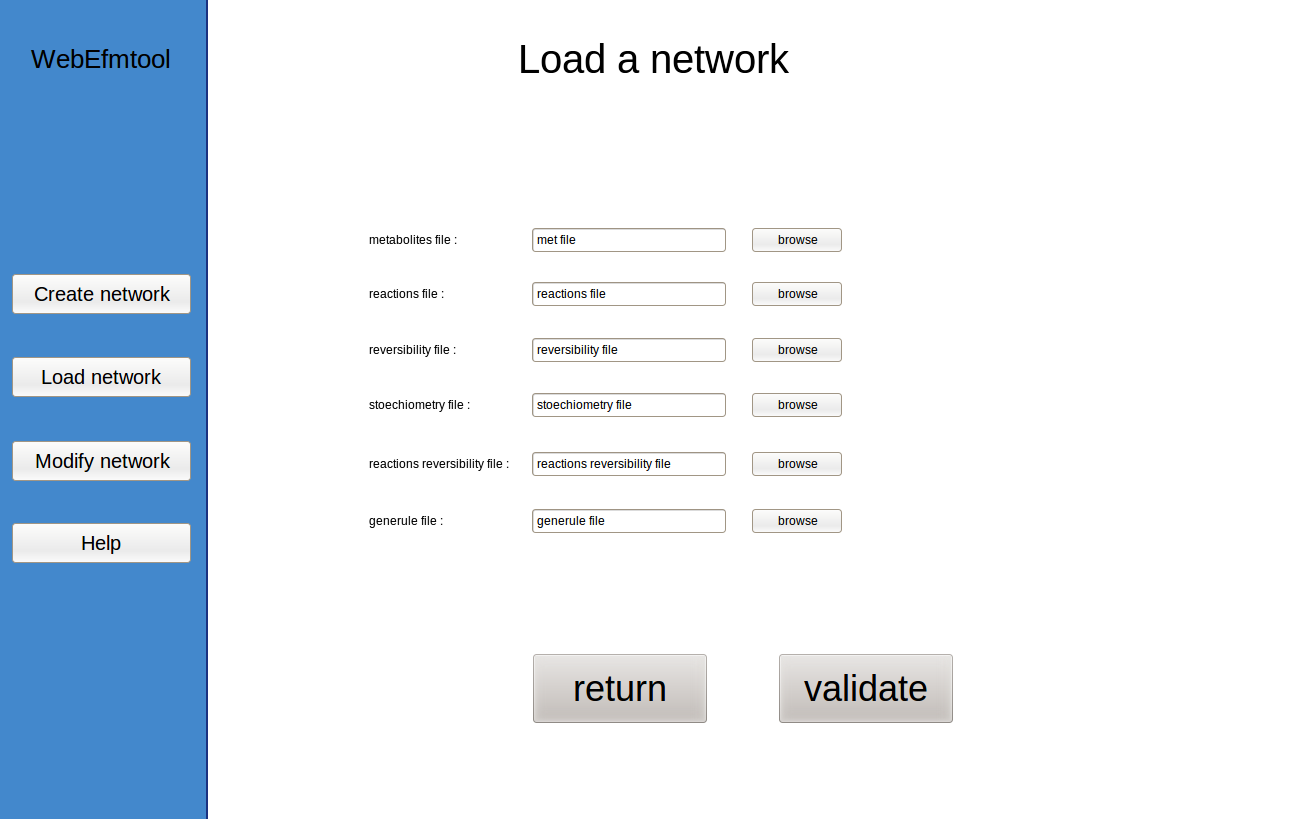
\includegraphics[width=0.90\textwidth]{Load.png}  
		 \end{minipage}}
		\caption{Chargement du réseau}
  		\label{chargement}
  	\end{center}	
\end{figure}

Si l'utilisateur clique sur le bouton de chargement d'un réseau depuis la page d'accueil, il devra charger une série de fichiers (depuis le disque dur de son ordinateur) nécessaires au bon fonctionnement de \textit{regEfmtool}. Les fichiers doivent être dans le format adéquat et un message d'erreur appara\^itra si ce n'est pas le cas. Au cas où, une fonction d'aide sera disponible pour avoir un modèle de fichiers à charger. 

\subsubsection{Lancement du programme}

\begin{figure}[!ht]
	\begin{center}
		\fbox{
   		 \begin{minipage}[c]{0.9\textwidth}
  			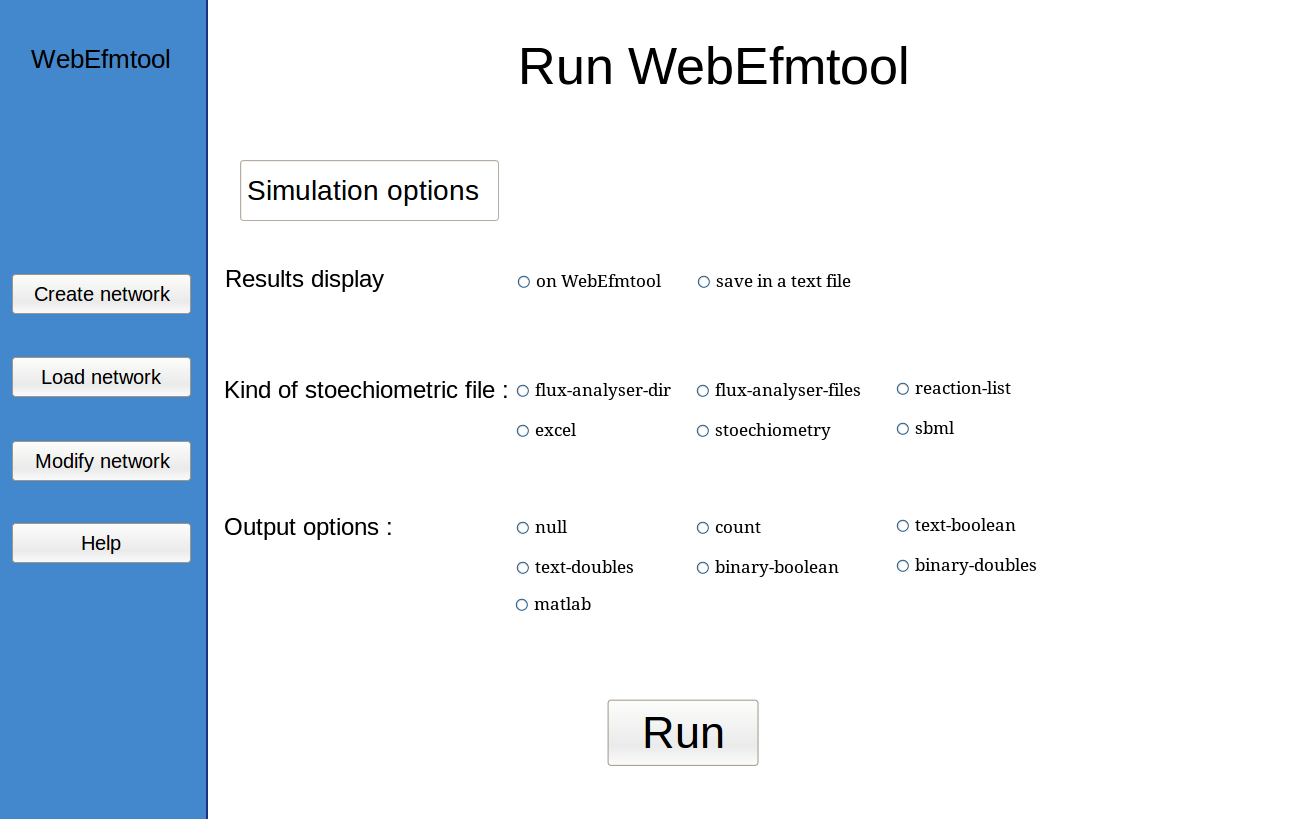
\includegraphics[width=0.90\textwidth]{Run.png}  
		 \end{minipage}}
		\caption{Lancement de RegEmftool}
  		\label{lancement}
  	\end{center}	
\end{figure}

Lorsque l'utilisateur aura créé son réseau manuellement ou l'aura chargé, il devra ensuite choisir les paramètres de calcul de \textit{regEfmtool}. Nous avons fait le choix d'utiliser des cases à cocher en fonction de ce qu'il choisira. Pour les utilisateurs non expérimentés, les choix de base seront pré-sélectionnés. Il suffira ensuite de cliquer sur le bouton "Run" pour avoir les résultats générés par le logiciel. Nous n'avons pas représenté toutes les options du lancement de \textit{regEfmtool} sur cette maquette, pour des raisons d'affichage.

\pagebreak

\section{Besoins non fonctionnels}

\subsection{Portabilité}
L'utilisation de \textit{regEfmtool} s'appuie sur d'autres logiciels, nécessitant par exemple la version 1.7 de Java. De ce fait, ils devront être libre d'utilisation pour le secteur académique. L'interface devra être livrée avec tous les fichiers de configuration (pré-existants ou nouvellement créés) et indépendante du système d'exploitation. 

\subsection{Sécurité et robustesse}
Il faudra gérer l'espace occupé par les fichier chargés sur le serveur. Le site devra être stable et gérer au mieux les erreurs qui pourraient être générées lors du chargement des fichiers, de la modification des paramètres ou des calculs. L'utilisateur sera donc informé en cas d'erreur lors du chargement d'un fichier non compatible avec \textit{regEfmtool}, contenant des erreurs d'écritures ou lorsque les paramètres entrés ne sont pas en accords avec la fonction ou l'option sélectionnée. 

\subsection{Temps de calcul}
Il faudra effectuer une vérification du nombre de métabolites et de réactions afin d'estimer le temps de calcul. Si ce dernier s'avère trop long, l'utilisateur sera prévenu et devra confirmer le lancement du processus. 

\subsection{Documentations}
L'écriture du code sera constituée de commentaires qui permettront la maintenance du code ainsi qu'une éventuelle amélioration de ce dernier par un tiers.
L'interface Web créée, quand à elle, devra être fournie avec une documentation sur son installation, son utilisation, sa maintenance et une charte graphique déclarant les différents attributs du site (couleurs utilisées, police, logo, image,...).

\subsection{Dates}
Début du projet mi-octobre 2012. \\
Remise du cahier des charges et présentation du sujet le 5 Décembre 2012.  \\
Mi-décembre 2012: point sur l'avancement du projet.\\
Rendez-vous pour l'avancement du code en janvier 2013.\\
Remise du projet mi-février 2013.